\documentclass{article}
\usepackage{fullpage}

%load needed packages
\usepackage{graphicx}
\usepackage{array}
\usepackage{booktabs}
\usepackage[utf8]{inputenc}
\usepackage[T1]{fontenc}

\usepackage[spanish]{babel} % Paquete para el idioma español

\usepackage{listings}
\usepackage{xcolor}

\definecolor{codegreen}{HTML}{5AB2FF}
\definecolor{morado}{HTML}{AD88C6}
\definecolor{BG}{HTML}{EEEEEE}
\definecolor{azul}{HTML}{4D869C}
\definecolor{sqlblue}{HTML}{FF8C00} % Color para las palabras clave SQL

% Estilo para DDL
\lstdefinestyle{ddlstyle}{
	language=SQL,
	backgroundcolor=\color{BG},
	commentstyle=\color{codegreen},
	basicstyle=\ttfamily\small,
	keywordstyle=\color{azul},
	stringstyle=\color{morado},
	showstringspaces=false,
	breaklines=true,
	frame=shadowbox,
	numbers=left,
	numberstyle=\tiny\color{gray},
	captionpos=b,
}

% Estilo para SQL
\lstdefinestyle{sqlstyle}{
	language=SQL,
	backgroundcolor=\color{BG},
	commentstyle=\color{codegreen},
	basicstyle=\ttfamily\small,
	keywordstyle=\color{sqlblue}, % Color diferente para palabras clave SQL
	stringstyle=\color{morado},
	showstringspaces=false,
	breaklines=true,
	frame=shadowbox,
	numbers=left,
	numberstyle=\tiny\color{gray},
	captionpos=b,
}

\begin{document}



% Portada
\begin{titlepage}
	\centering
	\vspace*{3cm}
	
	% Título destacado
	{\Huge \textbf{Practica 1: Bases De Datos Relacionales}\\[0.5cm]}
	
	% Espacio y logotipo (si lo tienes, por ejemplo el logo de tu universidad)
	\vspace{2cm}
	
\includegraphics[width=0.3\textwidth]{images/uma_logo.jpg}\\[1cm]
	
	% Nombre del autor
	{\LARGE \textbf{Alejandro Silva Rodríguez}\\[0.5cm]}
	{\LARGE \textbf{Marta Cuevas Rodríguez}\\[0.5cm]}
	{\large \textit{Almacenes De Datos}\\
		Universidad de Málaga\\
		}
	
	\vfill
	
	% Fecha en la parte inferior de la página
	{\large Septiembre 2024}
\end{titlepage}

% indice
\tableofcontents

\newpage

\section{Introducción}

En esta práctica, se diseñará y creará una base de datos para gestionar información sobre parques naturales en Andalucía y la liga española de fútbol de primera división. El objetivo es elaborar un modelo entidad-relación y un modelo relacional que muestren las características y relaciones de las entidades involucradas, utilizando herramientas de diseño de bases de datos.

Además, se generará el DDL (Data Definition Language) para SQL Server, que permitirá crear la base de datos y las tablas necesarias. Se incluirán datos sobre los parques naturales, su gestión y las especies que los habitan, así como información sobre los equipos de fútbol, sus jugadores y los partidos.

Este ejercicio ayudará a aplicar los conceptos de bases de datos y ofrecerá una experiencia práctica en el uso de herramientas y lenguajes de consulta.



\section{Parques Naturales}

En esta sección se explicara como se diseñó e implementó la base de datos de parques naturales y las consultas sobre la misma.

\subsection{Requisitos De Datos}

La Junta de Andalucía desea mantener la información sobre los parques naturales que hay en su comunidad autónoma. En particular sería necesario conocer el nombre del parque (que es único), su teléfono, dirección administrativa, una dirección web, un correo electrónico, su fecha de declaración como parque natural, la extensión (en hectáreas) de cada zona protegida, las especies animales que contiene, la población estimada de cada una de ellas y la dirección gestora del parque. Esta dirección gestora del parque está coordinada por un presidente y un número no determinado de consejeros. De todos estos miembros de la dirección gestora se desea conocer el DNI, nombre, fecha de nacimiento, dirección y teléfono de cada uno de ellos. Cada persona puede ser a lo sumo consejero en un parque y presidente de otro. De las especies guardamos su nombre científico y el común (ambos son únicos), el número de años de vida media. 
\\

Con objeto de poder determinar el estado de salud del parque necesitamos información sobre la interacción del hombre con el entorno. Para ello se almacenan datos sobre los municipios donde está ubicado el parque: número de municipios que abarca, nombre de cada uno de ellos, enlace a su web, fichero con la foto de su escudo, partido que gobierna en la alcaldía, número de habitantes y gasto de agua medio por habitante. 
\\

Las especies tienen una extensión (en hectáreas) necesaria para desarrollarse en libertad, dato que aparece en los estudios generales sobre cada especie. Sin embargo, el dato de si la especie está superpoblada en cada parque se guardará explícitamente, porque puede depender de factores como si el parque es montañoso, si tiene acuíferos, etc y por tanto precisa de la opinión última de un experto. Tenga en cuenta que cada municipio abarca a lo sumo un sólo parque. 

\subsection{Diseño Lógico}

\begin{figure}
	\centering
	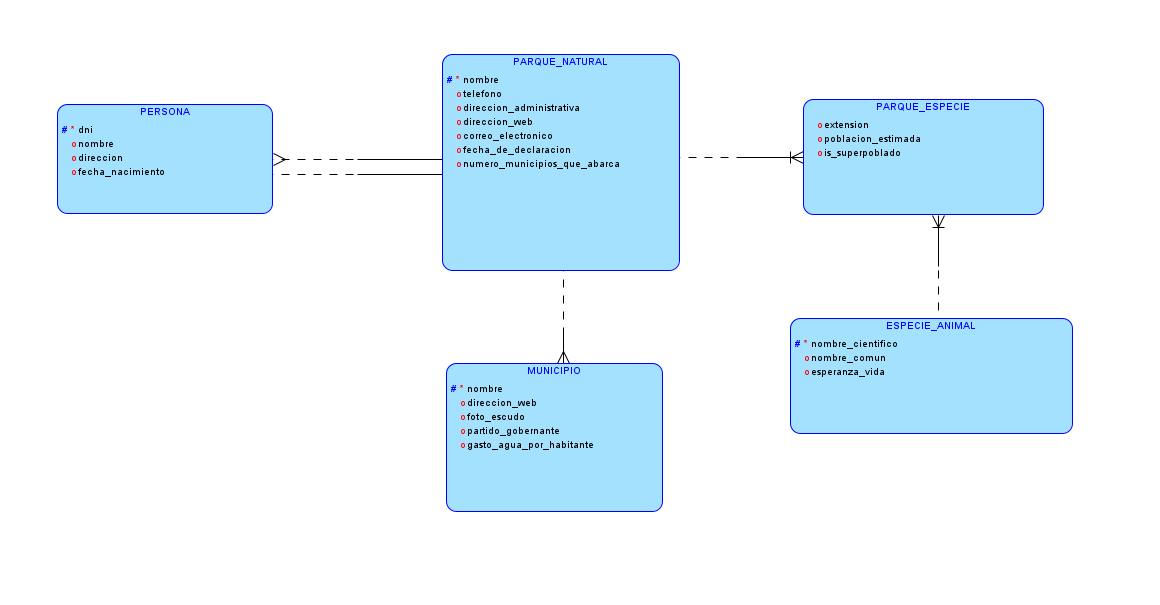
\includegraphics[width=0.70\textwidth]{images/diagrama_logico_parques_naturales.png}
	\caption{Diagrama Lógico De Parques Naturales}
	\label{fig:p_logico}
\end{figure}


\subsection{Diseño Entidad Relación}

\begin{figure}
	\centering
	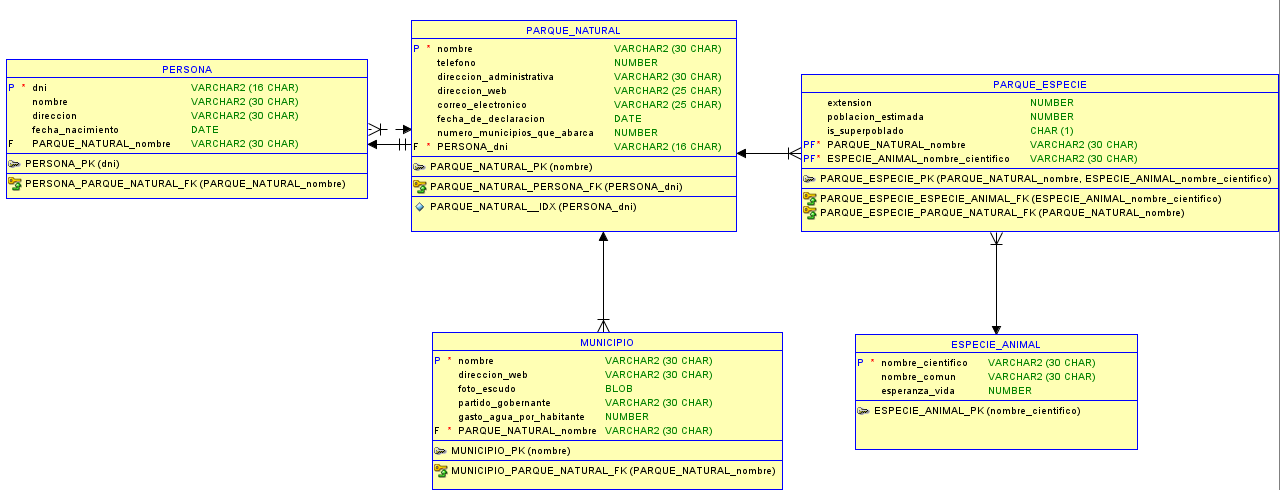
\includegraphics[width=0.70\textwidth]{images/diagrama_relacional_parques_naturales.png}
	\caption{Diagrama Relacional De Parques Naturales}
	\label{fig:p_relacional}
\end{figure}

\subsection{Implementación}

\begin{lstlisting}[style=ddlstyle, label=fig:p_ddl,caption=Definicion De Datos De Parques Naturales]
	
	CREATE TABLE ESPECIE_ANIMAL 
	(
	nombre_cientifico VARCHAR (30) NOT NULL , 
	nombre_comun VARCHAR (30) , 
	esperanza_vida NUMERIC (28) 
	)
	GO
	
	ALTER TABLE ESPECIE_ANIMAL ADD CONSTRAINT ESPECIE_ANIMAL_PK PRIMARY KEY CLUSTERED (nombre_cientifico)
	WITH (
	ALLOW_PAGE_LOCKS = ON , 
	ALLOW_ROW_LOCKS = ON )
	GO
	
	CREATE TABLE MUNICIPIO 
	(
	nombre VARCHAR (30) NOT NULL , 
	direccion_web VARCHAR (30) , 
	foto_escudo IMAGE , 
	partido_gobernante VARCHAR (30) , 
	gasto_agua_por_habitante NUMERIC (28) , 
	PARQUE_NATURAL_nombre VARCHAR (30) NOT NULL 
	)
	GO
	
	ALTER TABLE MUNICIPIO ADD CONSTRAINT MUNICIPIO_PK PRIMARY KEY CLUSTERED (nombre)
	WITH (
	ALLOW_PAGE_LOCKS = ON , 
	ALLOW_ROW_LOCKS = ON )
	GO
	
	CREATE TABLE PARQUE_ESPECIE 
	(
	extension NUMERIC (28) , 
	poblacion_estimada NUMERIC (28) , 
	is_superpoblado BIT , 
	PARQUE_NATURAL_nombre VARCHAR (30) NOT NULL , 
	ESPECIE_ANIMAL_nombre_cientifico VARCHAR (30) NOT NULL 
	)
	GO
	
	ALTER TABLE PARQUE_ESPECIE ADD CONSTRAINT PARQUE_ESPECIE_PK PRIMARY KEY CLUSTERED (PARQUE_NATURAL_nombre, ESPECIE_ANIMAL_nombre_cientifico)
	WITH (
	ALLOW_PAGE_LOCKS = ON , 
	ALLOW_ROW_LOCKS = ON )
	GO
	
	CREATE TABLE PARQUE_NATURAL 
	(
	nombre VARCHAR (30) NOT NULL , 
	telefono NUMERIC (28) , 
	direccion_administrativa VARCHAR (30) , 
	direccion_web VARCHAR (25) , 
	correo_electronico VARCHAR (25) , 
	fecha_de_declaracion DATE , 
	numero_municipios_que_abarca NUMERIC (28) , 
	PERSONA_dni VARCHAR (16) NOT NULL 
	)
	GO 
	
	
	
	
	CREATE UNIQUE NONCLUSTERED INDEX 
	PARQUE_NATURAL__IDX ON PARQUE_NATURAL 
	( 
	PERSONA_dni 
	) 
	GO
	
	ALTER TABLE PARQUE_NATURAL ADD CONSTRAINT PARQUE_NATURAL_PK PRIMARY KEY CLUSTERED (nombre)
	WITH (
	ALLOW_PAGE_LOCKS = ON , 
	ALLOW_ROW_LOCKS = ON )
	GO
	
	CREATE TABLE PERSONA 
	(
	dni VARCHAR (16) NOT NULL , 
	nombre VARCHAR (30) , 
	direccion VARCHAR (30) , 
	fecha_nacimiento DATE , 
	PARQUE_NATURAL_nombre VARCHAR (30) 
	)
	GO
	
	ALTER TABLE PERSONA ADD CONSTRAINT PERSONA_PK PRIMARY KEY CLUSTERED (dni)
	WITH (
	ALLOW_PAGE_LOCKS = ON , 
	ALLOW_ROW_LOCKS = ON )
	GO
	
	ALTER TABLE MUNICIPIO 
	ADD CONSTRAINT MUNICIPIO_PARQUE_NATURAL_FK FOREIGN KEY 
	( 
	PARQUE_NATURAL_nombre
	) 
	REFERENCES PARQUE_NATURAL 
	( 
	nombre 
	) 
	ON DELETE NO ACTION 
	ON UPDATE NO ACTION 
	GO
	
	ALTER TABLE PARQUE_ESPECIE 
	ADD CONSTRAINT PARQUE_ESPECIE_ESPECIE_ANIMAL_FK FOREIGN KEY 
	( 
	ESPECIE_ANIMAL_nombre_cientifico
	) 
	REFERENCES ESPECIE_ANIMAL 
	( 
	nombre_cientifico 
	) 
	ON DELETE NO ACTION 
	ON UPDATE NO ACTION 
	GO
	
	ALTER TABLE PARQUE_ESPECIE 
	ADD CONSTRAINT PARQUE_ESPECIE_PARQUE_NATURAL_FK FOREIGN KEY 
	( 
	PARQUE_NATURAL_nombre
	) 
	REFERENCES PARQUE_NATURAL 
	( 
	nombre 
	) 
	ON DELETE NO ACTION 
	ON UPDATE NO ACTION 
	GO
	
	ALTER TABLE PARQUE_NATURAL 
	ADD CONSTRAINT PARQUE_NATURAL_PERSONA_FK FOREIGN KEY 
	( 
	PERSONA_dni
	) 
	REFERENCES PERSONA 
	( 
	dni 
	) 
	ON DELETE NO ACTION 
	ON UPDATE NO ACTION 
	GO
	
	ALTER TABLE PERSONA 
	ADD CONSTRAINT PERSONA_PARQUE_NATURAL_FK FOREIGN KEY 
	( 
	PARQUE_NATURAL_nombre
	) 
	REFERENCES PARQUE_NATURAL 
	( 
	nombre 
	) 
	ON DELETE NO ACTION 
	ON UPDATE NO ACTION 
	GO

\end{lstlisting}

\begin{lstlisting}[style=sqlstyle, label=fig:p_insert,caption=Carga de datos]
	-- Insertar especies animales
	INSERT INTO ESPECIE_ANIMAL (nombre_cientifico, nombre_comun, esperanza_vida) VALUES
	('Ursus arctos', 'Oso pardo', 25),
	('Canis lupus', 'Lobo', 15),
	('Ailuropoda melanoleuca', 'Oso panda', 20),
	('Panthera leo', 'Leon', 14),
	('Elephas maximus', 'Elefante asiático', 60),
	('Giraffa camelopardalis', 'Jirafa', 25),
	('Balaenoptera musculus', 'Ballena azul', 80),
	('Puma concolor', 'Puma', 12),
	('Carcharodon carcharias', 'Tiburón blanco', 30),
	('Lycaon pictus', 'Perro salvaje africano', 10),
	('Lynx pardinus', 'Lynx ibérico', 13),
	('Acinonyx jubatus', 'Guepardo', 12),
	('Aquila chrysaetos', 'Águila real', 30),
	('Haliaeetus leucocephalus', 'Águila calva', 20),
	('Dendrocopos major', 'Pico picapinos', 10);
	
	-- Insertar personas (presidentes) - un presidente por parque natural
	INSERT INTO PERSONA (dni, nombre, direccion, fecha_nacimiento) VALUES
	('12345678A', 'Juan Pérez', 'Calle Falsa 123', '1980-01-01'),  -- Sierra Nevada
	('23456789B', 'María García', 'Avenida Real 456', '1990-05-15'),  -- Doñana
	('34567890C', 'Luis Torres', 'Calle Larga 789', '1985-02-20'),  -- Cabo de Gata
	('45678901D', 'Ana Martínez', 'Plaza Central 321', '1992-08-22');  -- Picos de Europa
	
	-- Insertar parques naturales
	INSERT INTO PARQUE_NATURAL (nombre, telefono, direccion_administrativa, direccion_web, correo_electronico, fecha_de_declaracion, numero_municipios_que_abarca, PERSONA_dni) VALUES
	('Sierra Nevada', 123456789, 'Granada', 'www.sierranevada.com', 'contacto@sierranevada.com', '1989-06-01', 0, '12345678A'),
	('Doñana', 987654321, 'Huelva', 'www.donana.com', 'contacto@donana.com', '1994-07-15', 0, '23456789B'),
	('Cabo de Gata', 123123123, 'Almería', 'www.cabodegata.com', 'info@cabodegata.com', '1997-05-12', 0, '34567890C'),
	('Picos de Europa', 321321321, 'Asturias', 'www.picosdeeuropa.com', 'contacto@picos.com', '1999-10-05', 0, '45678901D');
	
	-- Insertar consejeros
	INSERT INTO PERSONA (dni, nombre, direccion, fecha_nacimiento, PARQUE_NATURAL_nombre) VALUES
	
	('89012345H', 'Elena Ruiz', 'Avenida del Parque 654', '1983-08-12', 'Doñana'),
	('90123456I', 'Fernando García', 'Calle del Río 765', '1990-01-25', 'Doñana'),
	('12345678J', 'Fernando Pérez', 'Calle Vista 123', '1982-05-05', 'Cabo de Gata'),
	('23456789K', 'Valeria Torres', 'Avenida Costa 234', '1988-09-17', 'Cabo de Gata'),
	('34567890L', 'Diego Castillo', 'Calle Playa 345', '1993-12-20', 'Cabo de Gata'),
	('45678901M', 'Rosa Medina', 'Plaza de la Paz 456', '1995-04-08', 'Cabo de Gata'),
	('56789012N', 'Hugo Jiménez', 'Calle del Sol 567', '1990-11-01', 'Cabo de Gata'),
	('67890123O', 'Carmen Romero', 'Avenida Montaña 678', '1994-03-13', 'Picos de Europa'),
	('78901234P', 'Salvador Gómez', 'Calle Viento 789', '1981-02-25', 'Picos de Europa'),
	('89012345Q', 'Marina González', 'Calle Nieve 890', '1986-07-05', 'Picos de Europa'),
	('90123456R', 'Luis Méndez', 'Avenida Río 901', '1978-01-15', 'Picos de Europa'),
	('01234567S', 'Natalia Ortiz', 'Calle Bosque 012', '1990-10-19', 'Picos de Europa');
	go
	-- Actualizar el numero de municipios del parque al insertar un municipio al que pertenece
	CREATE TRIGGER actualizar_numero_municipios_insert
	ON MUNICIPIO
	AFTER INSERT
	AS
	BEGIN
	-- Sumar 1 a cada parque natural por cada municipio insertado
	UPDATE PN
	SET PN.numero_municipios_que_abarca = PN.numero_municipios_que_abarca + (
	SELECT COUNT(*)
	FROM inserted I
	WHERE I.PARQUE_NATURAL_nombre = PN.nombre
	)
	FROM PARQUE_NATURAL PN
	WHERE EXISTS (
	SELECT 1 FROM inserted I WHERE I.PARQUE_NATURAL_nombre = PN.nombre
	);
	END;
	GO
	
	
	CREATE TRIGGER actualizar_numero_municipios_delete
	ON MUNICIPIO
	AFTER DELETE
	AS
	BEGIN
	-- Restar 1 a cada parque natural por cada municipio eliminado
	UPDATE PN
	SET PN.numero_municipios_que_abarca = PN.numero_municipios_que_abarca - (
	SELECT COUNT(*)
	FROM deleted D
	WHERE D.PARQUE_NATURAL_nombre = PN.nombre
	)
	FROM PARQUE_NATURAL PN
	WHERE EXISTS (
	SELECT 1 FROM deleted D WHERE D.PARQUE_NATURAL_nombre = PN.nombre
	);
	END;
	GO
	
	-- Insertar municipios
	INSERT INTO MUNICIPIO (nombre, direccion_web, foto_escudo, partido_gobernante, gasto_agua_por_habitante, PARQUE_NATURAL_nombre) VALUES
	('Granada', 'www.granada.es', NULL, 'PSOE', 50.25, 'Sierra Nevada'),
	('Almonte', 'www.almonte.es', NULL, 'PP', 60.50, 'Doñana'),
	('Almería', 'www.almeria.es', NULL, 'C’s', 55.00, 'Cabo de Gata'),
	('Cangas de Onís', 'www.cangasdeonis.es', NULL, 'PSOE', 45.75, 'Picos de Europa'),
	('Baza', 'www.baza.es', NULL, 'PP', 58.25, 'Sierra Nevada'),
	('Huelva', 'www.huelva.es', NULL, 'PSOE', 57.00, 'Doñana'),
	('Oviedo', 'www.oviedo.es', NULL, 'PSOE', 62.00, 'Picos de Europa'),
	('San José', 'www.sanjose.es', NULL, 'PP', 61.50, 'Cabo de Gata'),
	('La Zubia', 'www.lazubia.es', NULL, 'PSOE', 54.00, 'Sierra Nevada'),
	('Moguer', 'www.moguer.es', NULL, 'PP', 59.00, 'Doñana');
	
	-- Insertar especies en parques
	INSERT INTO PARQUE_ESPECIE (extension, poblacion_estimada, is_superpoblado, PARQUE_NATURAL_nombre, ESPECIE_ANIMAL_nombre_cientifico) VALUES
	(10000, 200, 0, 'Sierra Nevada', 'Ursus arctos'),
	(15000, 150, 0, 'Doñana', 'Canis lupus'),
	(12000, 50, 1, 'Doñana', 'Ailuropoda melanoleuca'),
	(13000, 300, 0, 'Cabo de Gata', 'Giraffa camelopardalis'),
	(14000, 250, 0, 'Picos de Europa', 'Panthera leo'),
	(8000, 100, 0, 'Cabo de Gata', 'Elephas maximus'),
	(9000, 60, 0, 'Sierra Nevada', 'Balaenoptera musculus'),
	(11000, 80, 1, 'Doñana', 'Puma concolor'),
	(10000, 500, 0, 'Picos de Europa', 'Lynx pardinus'),
	(9000, 75, 0, 'Cabo de Gata', 'Acinonyx jubatus'),
	(15000, 120, 0, 'Sierra Nevada', 'Aquila chrysaetos'),
	(16000, 200, 0, 'Picos de Europa', 'Haliaeetus leucocephalus'),
	(17000, 90, 0, 'Doñana', 'Dendrocopos major');
	
	
\end{lstlisting}
\subsection{Consultas}

\begin{lstlisting}[style=sqlstyle, label=fig:p_consultas,caption=Consultas Sobre Parques Naturales]
	
	 use parques_naturales
	go
	
	-- Consulta 1: Seleccionar los animales que se pueden encontrar en Sierra Nevada
	
	SELECT e.nombre_cientifico, e.nombre_comun, p.nombre
	FROM PARQUE_NATURAL p , PARQUE_ESPECIE pe, ESPECIE_ANIMAL e
	WHERE e.nombre_cientifico=pe.ESPECIE_ANIMAL_nombre_cientifico and pe.PARQUE_NATURAL_nombre=p.nombre and p.nombre='Sierra Nevada';
	
	-- Consulta 2: Seleccionar el nombre de los consejeros de Doñana
	
	SELECT p.nombre, c.nombre
	FROM PARQUE_NATURAL p, PERSONA c
	WHERE c.PARQUE_NATURAL_nombre=p.nombre and p.nombre='Doñana';
	
	-- Consulta 3: Seleccionar el nombre del presidente de Doñana
	
	SELECT p.nombre, c.nombre
	FROM PARQUE_NATURAL p, PERSONA c
	WHERE c.dni=p.PERSONA_dni and p.nombre='Doñana';
	
	-- Consulta 4: Seleccionar el nombre de los municipios que abarca doñana junto al numero de municipios que abarca
	
	SELECT m.nombre, p.nombre, p.numero_municipios_que_abarca
	FROM PARQUE_NATURAL p, MUNICIPIO m
	WHERE p.nombre=m.PARQUE_NATURAL_nombre and p.nombre='Doñana';
	
	-- Consulta 5: Seleccionar el nombre de los presidentes de paruqes en los que se encuentra algun tipo de oso
	
	SELECT e.nombre_comun, presi.nombre, p.nombre
	FROM PERSONA presi, ESPECIE_ANIMAL e, PARQUE_NATURAL p, PARQUE_ESPECIE pe
	WHERE presi.dni=p.PERSONA_dni and p.nombre=pe.PARQUE_NATURAL_nombre and pe.ESPECIE_ANIMAL_nombre_cientifico=e.nombre_cientifico and e.nombre_comun LIKE 'Oso%';
  \end{lstlisting}
\section{Liga De Futbol}

Lorem ipsum dolor sit amet, consectetur adipiscing elit, sed do eiusmod tempor incididunt ut labore et dolore magna aliqua. Ut enim ad minim veniam, quis nostrud exercitation ullamco laboris nisi ut aliquip ex ea commodo consequat. Duis aute irure dolor in reprehenderit in voluptate velit esse cillum dolore eu fugiat nulla pariatur. Excepteur sint occaecat cupidatat non proident, sunt in culpa qui officia deserunt mollit anim id est laborum.


Reference Figure \ref{fig:example1}.

\cite{oracle2024}
\cite{sqlserver2022}

% Incluir la bibliografía
\bibliographystyle{plain}  % Estilo de la bibliografía (por ejemplo, plain, alpha, ieee, etc.)
\bibliography{biblio}  % Nombre del archivo .bib sin la extensión

\end{document}
